\documentclass{standalone}
\usepackage{tikz}
\usetikzlibrary[arrows,positioning,matrix]

\begin{document}
\begin{tikzpicture}
  \node[draw=none] (posturesessions) {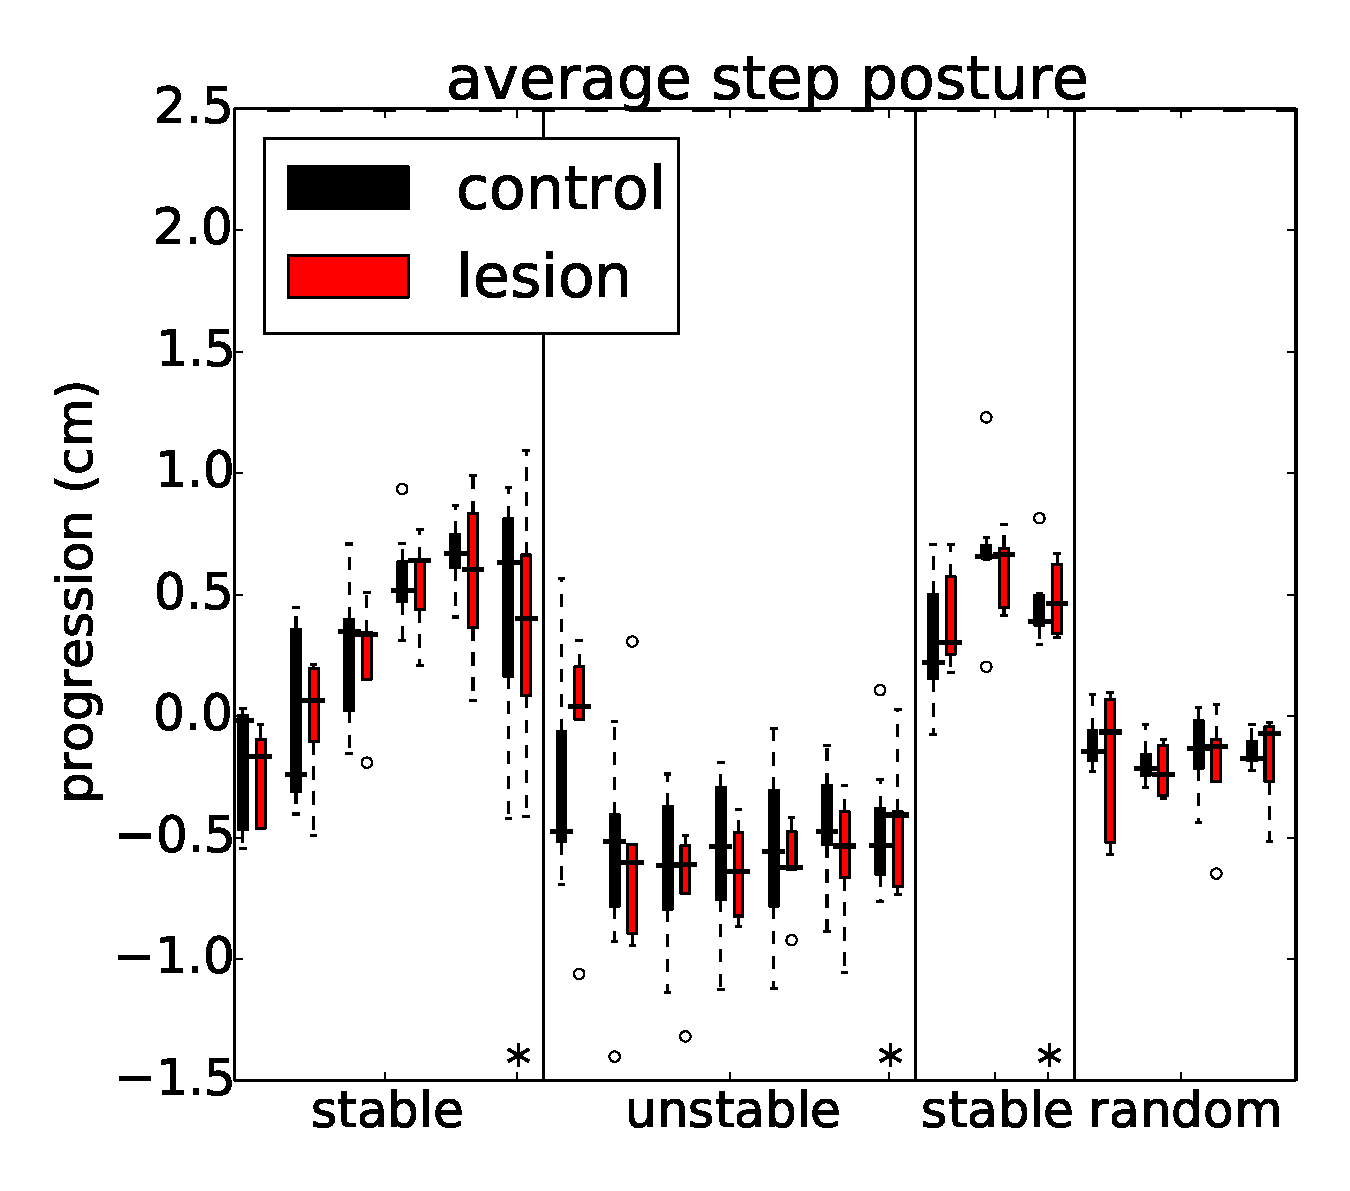
\includegraphics[width=0.5\textwidth]{elements/posturesessions}};
  \node[draw=none,above left=-3.5mm and -6.5mm of posturesessions] {A};

  \node[draw=none,right=1mm of posturesessions] (posturespeed) {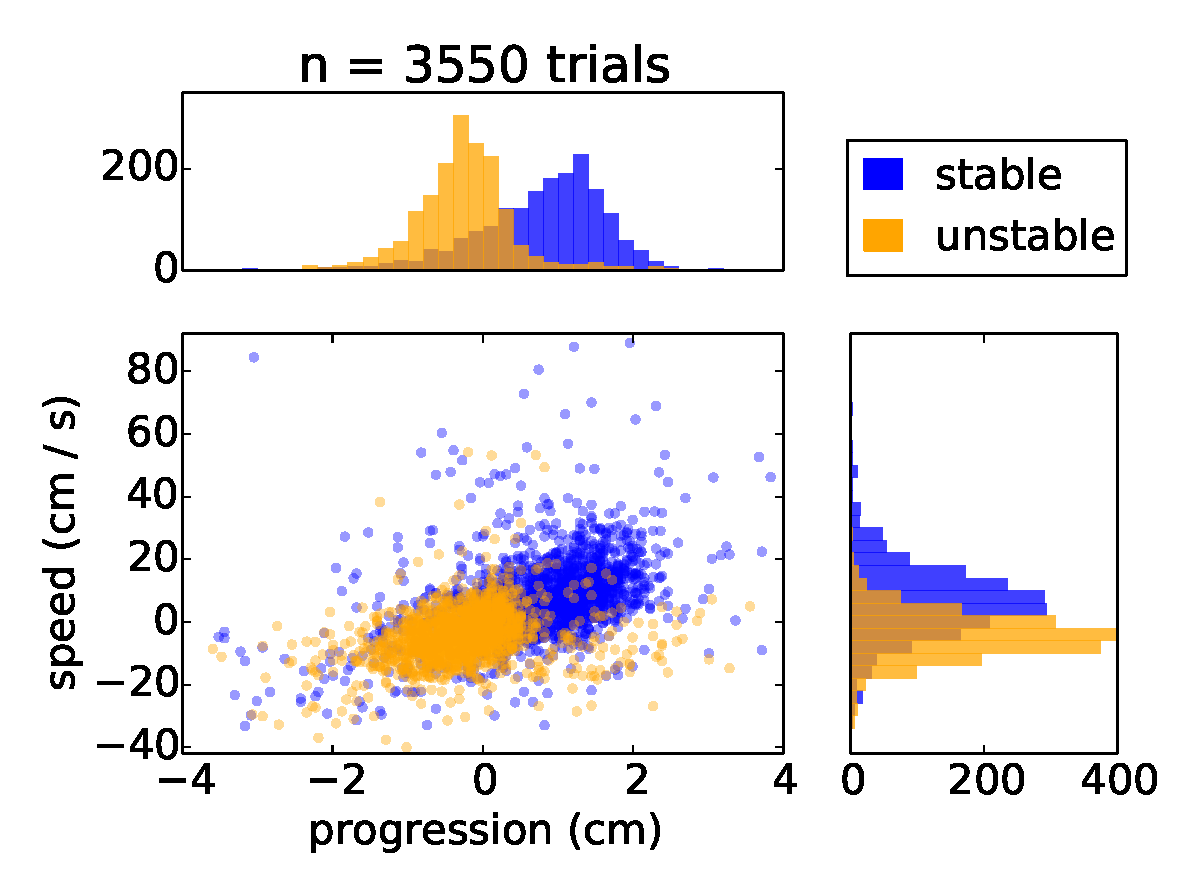
\includegraphics[width=0.5\textwidth]{elements/speedhistograms_b}};
  \node[draw=none,above=-2mm of posturespeed] {};
  \node[draw=none,above left=0.75mm and -5.5mm of posturespeed] {B};
  
  \node[draw=none,below=5mm of posturesessions] (posturesmalllesions) {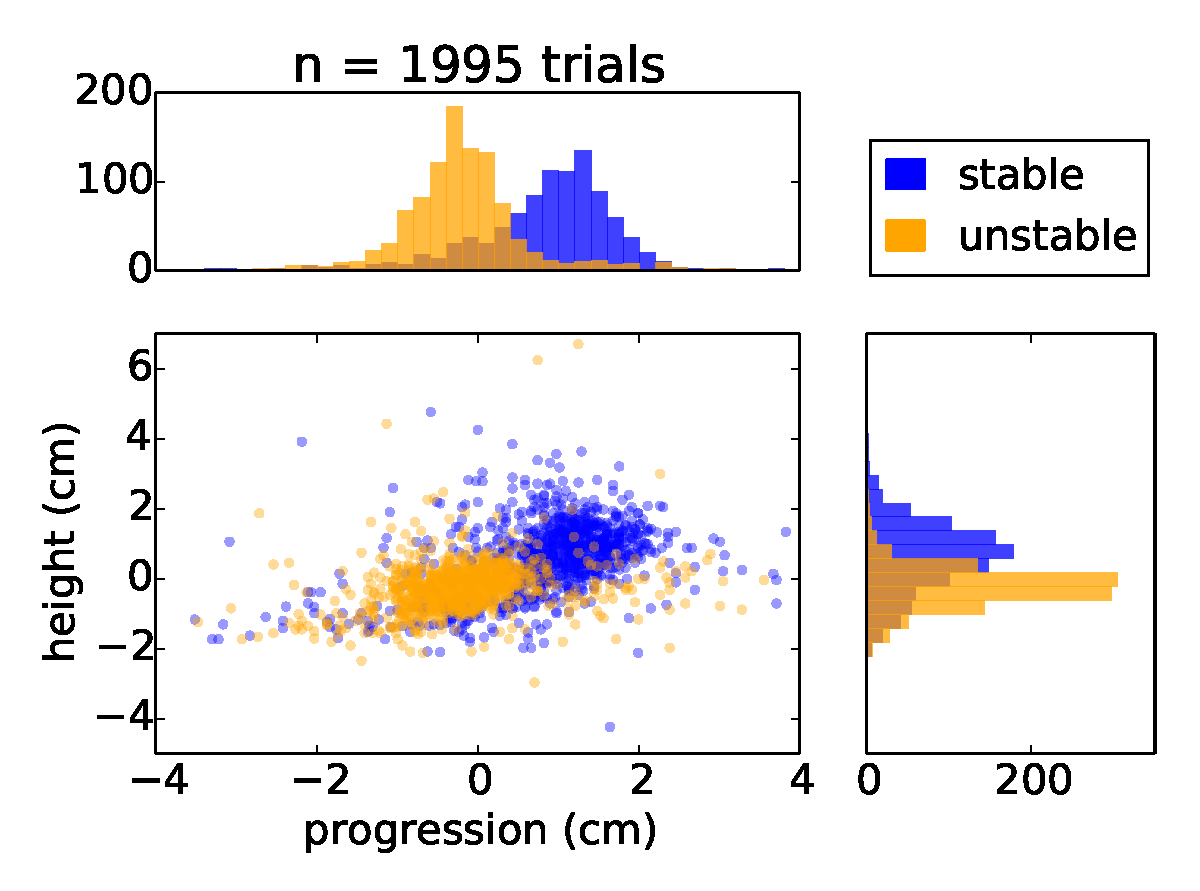
\includegraphics[width=0.5\textwidth]{elements/posturehistograms_controls_c}};
  \node[draw=none,above=-2mm of posturesmalllesions] {controls};
  \node[draw=none,above left=-2.5mm and -6mm of posturesmalllesions] {C};
  
  \node[draw=none,right=1mm of posturesmalllesions] (posturelesions) {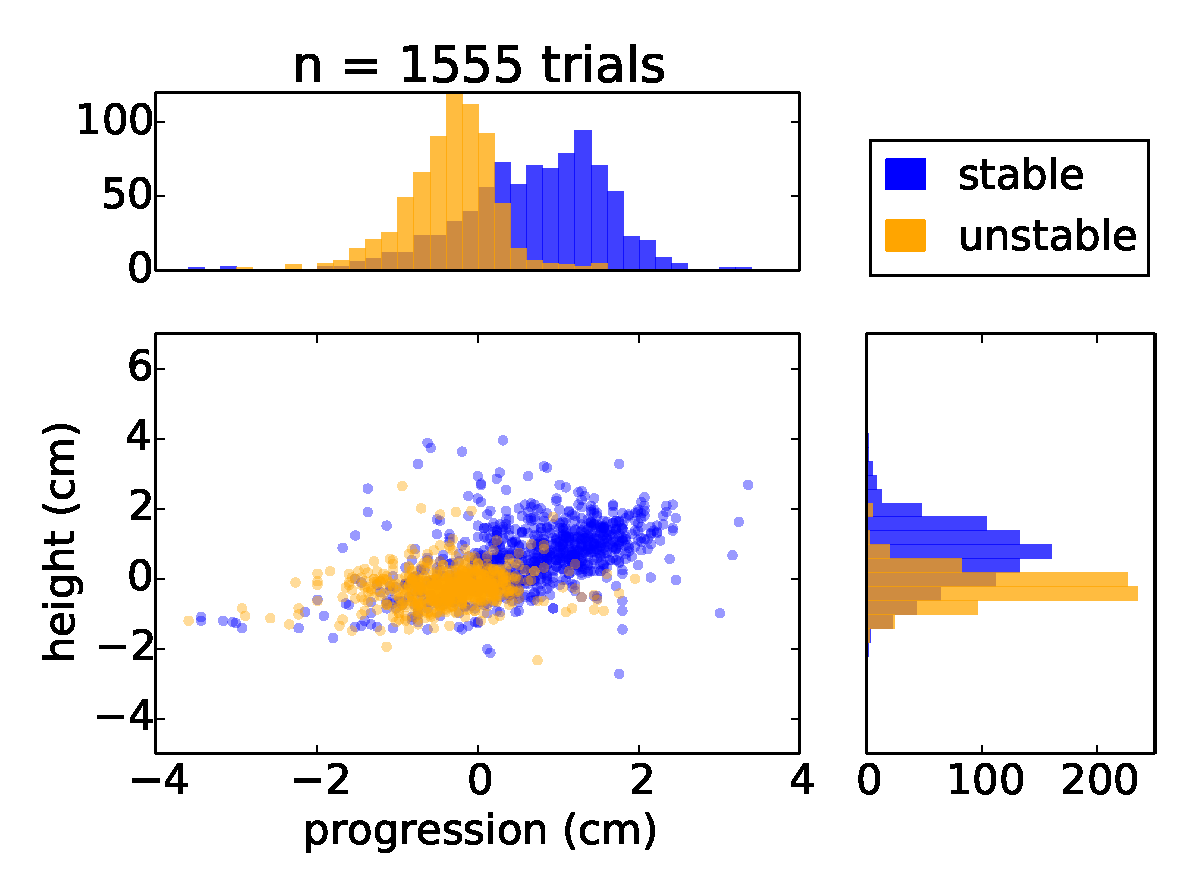
\includegraphics[width=0.5\textwidth]{elements/posturehistograms_alllesions_c}};
  \node[draw=none,above=-2.5mm of posturelesions] {lesions};
  \node[draw=none,above left=-2.5mm and -6mm of posturelesions] {D};
\end{tikzpicture}
\end{document}